\documentclass[../main.tex]{subfiles}

\begin{document}

\part{Curve Fitting}

\section{OVERVIEW}

\noindent \textbf{What Is Curve Fitting?}

\noindent Data are often given for discrete values along a continuum. However, you may require estimates at points between the discrete values. Chapters 14 through 18 describe techniques to
fit curves to such data to obtain intermediate estimates. In addition, you may require a simplified version of a complicated function. One way to do this is to compute values of the
function at a number of discrete values along the range of interest. Then, a simpler function
may be derived to fit these values. Both of these applications are known as \textit{curve fitting}.

There are two general approaches for curve fitting that are distinguished from each
other on the basis of the amount of error associated with the data. First, where the data
exhibit a significant degree of error or ``scatter,'' the strategy is to derive a single curve that
represents the general trend of the data. Because any individual data point may be incorrect, we make no effort to intersect every point. Rather, the curve is designed to follow the
pattern of the points taken as a group. One approach of this nature is called \textit{least-squares
regression} (Fig. PT4.1a).

Second, where the data are known to be very precise, the basic approach is to fit a
curve or a series of curves that pass directly through each of the points. Such
data usually originate from tables. Examples are values for the density of water
or for the heat capacity of gases as a
function of temperature. The estimation
of values between well-known discrete
points is called \textit{interpolation} (Fig.
PT4.1b and c).

\noindent \textbf{Curve Fitting and Engineering and
Science. }  Your first exposure to curve
fitting may have been to determine intermediate values from tabulated data- for instance, from interest tables for
engineering economics or from steam tables for thermodynamics. Throughout the remainder of your career, you will have frequent occasion to estimate intermediate values from such tables.

\begin{figure}[H]
	\centering
	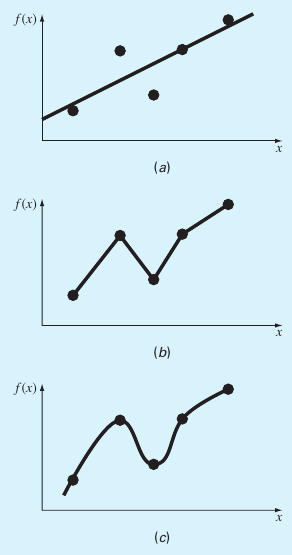
\includegraphics[width=1\linewidth]{fig_4_1pt}
	\caption{\textsf{Three attempts to fit a ``best'' curve through five data points: (a) least-squares regression, (b) linear
	interpolation, and (c) curvilinear interpolation.}}
	\label{fig:fig_4_1pt}
\end{figure}

Although many of the widely used engineering and scientific properties have been tabulated, there are a great many more that are not available in this convenient form. Special
cases and new problem contexts often require that you measure your own data and develop
your own predictive relationships. Two types of applications are generally encountered
when fitting experimental data: trend analysis and hypothesis testing.

\textit{Trend analysis} represents the process of using the pattern of the data to make predictions. For cases where the data are measured with high precision, you might utilize interpolating polynomials. Imprecise data are often analyzed with least-squares regression.

Trend analysis may be used to predict or forecast values of the dependent variable. This
can involve extrapolation beyond the limits of the observed data or interpolation within the
range of the data. All fields of engineering and science involve problems of this type.

A second application of experimental curve fitting is \textit{hypothesis testing}. Here, an
existing mathematical model is compared with measured data. If the model coefficients are unknown, it may be necessary to determine values that best fit the observed data. On the
other hand, if estimates of the model coefficients are already available, it may be appropriate to compare predicted values of the model with observed values to test the adequacy of
the model. Often, alternative models are compared and the ``best'' one is selected on the
basis of empirical observations.

In addition to the foregoing engineering and scientific applications, curve fitting is important in other numerical methods such as integration and the approximate solution of differential equations. Finally, curve-fitting techniques can be used to derive simple functions
to approximate complicated functions.

\section{PART ORGANIZATION}

\noindent After a brief review of statistics, Chap. 14 focuses on \textit{linear regression}; that is, how to determine the ``best'' straight line through a set of uncertain data points. Besides discussing how to
calculate the slope and intercept of this straight line, we also present quantitative and visual
methods for evaluating the validity of the results. In addition, we describe \textit{random number
generation} as well as several approaches for the linearization of nonlinear equations.

Chapter 15 begins with brief discussions of polynomial and multiple linear regression.
\textit{Polynomial regression} deals with developing a best fit of parabolas, cubics, or higher-order
polynomials. This is followed by a description of \textit{multiple linear regression}, which is designed for the case where the dependent variable $y$ is a linear function of two or more
independent variables $x_1, x_2, \dots , x_m$. This approach has special utility for evaluating experimental data where the variable of interest is dependent on a number of different factors.

After multiple regression, we illustrate how polynomial and multiple regression are
both subsets of a \textit{general linear least-squares model}. Among other things, this will allow
us to introduce a concise matrix representation of regression and discuss its general statistical properties. Finally, the last sections of Chap. 15 are devoted to \textit{nonlinear regression}.
This approach is designed to compute a least-squares fit of a nonlinear equation to data.

\textit{Chapter 16} deals with \textit{Fourier analysis} which involves fitting periodic functions to
data. Our emphasis will be on the \textit{fast Fourier transform} or \textit{FFT}. This method, which is
readily implemented with MATLAB, has many engineering applications, ranging from
vibration analysis of structures to signal processing.

In \textit{Chap. 17}, the alternative curve-fitting technique called \textit{interpolation} is described.
As discussed previously, interpolation is used for estimating intermediate values between
precise data points. In Chap. 17, polynomials are derived for this purpose. We introduce the
basic concept of polynomial interpolation by using straight lines and parabolas to connect
points. Then, we develop a generalized procedure for fitting an nth-order polynomial. Two
formats are presented for expressing these polynomials in equation form. The first, called
\textit{Newton's interpolating polynomial}, is preferable when the appropriate order of the polynomial is unknown. The second, called the \textit{Lagrange interpolating polynomial}, has advantages when the proper order is known beforehand.

Finally, \textit{Chap. 18} presents an alternative technique for fitting precise data points. This
technique, called \textit{spline interpolation}, fits polynomials to data but in a piecewise fashion.
As such, it is particularly well suited for fitting data that are generally smooth but exhibit
abrupt local changes. The chapter ends with an overview of how piecewise interpolation is
implemented in MATLAB.






\blankpage


\end{document}